\documentclass[10pt, a4paper]{article}

\usepackage{dingbat}          % \checkmark
\usepackage[table]{xcolor}

\usepackage{amsmath}          % Zaawansowana obróbka wzorów matematycznych
\usepackage{graphicx}         % Kolorowanie tekstu
%\usepackage{multicol}         % ?
\usepackage{multirow}
%\usepackage[makeroom]{cancel} % ?
\usepackage{polski}           % Polskie znaki
\usepackage[utf8]{inputenc}   % Kodowanie UTF8
\usepackage{geometry}         % Ustawienia układu strony dokumentu
 \geometry{
 a4paper,
 % width  = totalx - left
 % height = totaly - top
 total={180mm,267mm},
 left=15mm,
 top=15mm,
 }

\begin{document}

\begin{flushright}
    Kacper Kowalik (277646) \\
    Adam Matysiak (277641)
\end{flushright}

\vspace{2mm}

\begin{center}
    Fizyka 3.1 - Laboratorium \\
    \vspace{15px}
    {\Large{\textbf{
    Wyznaczanie współczynnika rozszerzalności termicznej\\
    oraz badanie procesów przekazywania ciepła
    }}} \\
    \vspace{15px}
    Ćwiczenie 29 \\
\end{center}
    
\begin{flushright}
    \begin{tabular}{lr}
         Data wykonania ćwiczenia:  & 18.04.2024 \\
         Data oddania sprawozdania: & 25.04.2024
    \end{tabular}
\end{flushright}


{\section{Spis przyrządów}}

\begin{itemize}
    \item Omomierz AGILENT 34401A,
    \item Omomierz analogowy Axiomet AX-7003,
    \item Rezystory wzorcowe 1$\Omega$, 10$\Omega$, 10k$\Omega$,
    \item Rezystory na płytce 220k$\Omega$, 6.8k$\Omega$, 100$\Omega$,
    \item Rezystor mocy 2.2k$\Omega$,
    \item Zasilacz nieregulowany
\end{itemize}

{\section{Przebieg i cel ćwiczenia}}

Ćwiczenie polegało na pomiarach rezystancji dostępnych na stanowisku rezystorów za pomocą różnych metod i układów pomiarowych takich jak: ukłda dwupunktowy, układ czteropunktowy, układ poprawnego pomiaru napięcia oraz poprawnego pomiaru prądu, a następnmie porównaniu ich z wartościami odczytanymi z rezystorów. W ćwiczeniu mieliśmy także za zadanie sprawdzić oddziaływanie przewodów pomiarowych na dokładność pomiaru. \\


\newpage
\section{Wyniki i analiza pomiarów}

% ⠀⠀⠀⠀⠀⠀⠀⠀⠀⠀⠀⠀⠀⠀⠀⠀⠀⠀⠀⣀⣤⣤⣤⣶⣤⣤⣀⣀⣀⠀⠀⠀⠀⠀⠀⠀⠀⠀⠀⠀⠀⠀⠀⠀⠀⠀⠀⠀⠀⠀
%⠀⠀⠀⠀⠀⠀⠀⠀⠀⠀⠀⠀⠀⠀⠀⠀⣠⣴⣿⣿⣿⣿⣿⣿⣿⣿⣿⣿⣿⣿⣶⣄⠀⠀⠀⠀⠀⠀⠀⠀⠀⠀⠀⠀⠀⠀⠀⠀⠀⠀
%⠀⠀⠀⠀⠀⠀⠀⠀⠀⠀⠀⠀⠀⠀⢀⣾⣿⣿⣿⣿⣿⡿⠋⠉⠛⠛⠛⠿⣿⠿⠿⢿⣇⠀⠀⠀⠀⠀⠀⠀⠀⠀⠀⠀⠀⠀⠀⠀⠀⠀
%⠀⠀⠀⠀⠀⠀⠀⠀⠀⠀⠀⠀⠀⠀⣾⣿⣿⣿⣿⣿⠟⠀⠀⠀⠀⠀⡀⢀⣽⣷⣆⡀⠙⣧⠀⠀⠀⠀⠀⠀⠀⠀⠀⠀⠀⠀⠀⠀⠀⠀
%⠀⠀⠀⠀⠀⠀⠀⠀⠀⠀⠀⠀⠀⢰⣿⣿⣿⣿⣿⣷⠶⠋⠀⠀⣠⣤⣤⣉⣉⣿⠙⣿⠀⢸⡆⠀⠀⠀⠀⠀⠀⠀⠀⠀⠀⠀⠀⠀⠀⠀
%⠀⠀⠀⠀⠀⠀⠀⠀⠀⠀⠀⠀⠀⢸⣿⣿⣿⣿⣿⠁⠀⠀⠴⡟⣻⣿⣿⣿⣿⣿⣶⣿⣦⡀⣇⠀⠀⠀⠀⠀⠀⠀⠀⠀⠀⠀⠀⠀⠀⠀
%⠀⠀⠀⠀⠀⠀⠀⠀⠀⠀⠀⠀⠀⢨⠟⡿⠻⣿⠃⠀⠀⠀⠻⢿⣿⣿⣿⣿⣿⠏⢹⣿⣿⣿⢿⡇⠀⠀⠀⠀⠀⠀⠀⠀⠀⠀⠀⠀⠀⠀
%⠀⠀⠀⠀⠀⠀⠀⠀⠀⠀⠀⠀⠀⣿⣼⣷⡶⣿⣄⠀⠀⠀⠀⠀⢉⣿⣿⣿⡿⠀⠸⣿⣿⡿⣷⠃⠀⠀⠀⠀⠀⠀⠀⠀⠀⠀⠀⠀⠀⠀
%⠀⠀⠀⠀⠀⠀⠀⠀⠀⠀⠀⠀⠀⢻⡿⣦⢀⣿⣿⣄⡀⣀⣰⠾⠛⣻⣿⣿⣟⣲⡀⢸⡿⡟⠹⡆⠀⠀⠀⠀⠀⠀⠀⠀⠀⠀⠀⠀⠀⠀
%⠀⠀⠀⠀⠀⠀⠀⠀⠀⠀⠀⠀⠀⠀⢰⠞⣾⣿⡛⣿⣿⣿⣿⣰⣾⣿⣿⣿⣿⣿⣿⣿⣿⡇⢰⡇⠀⠀⠀⠀⠀⠀⠀⠀⠀⠀⠀⠀⠀⠀
%⠀⠀⠀⠀⠀⠀⠀⠀⠀⠀⠀⠀⠀⠀⠘⠀⣿⡽⢿⣿⣿⣿⣿⣿⣿⣿⣿⣿⣿⢿⠿⣍⣿⣧⡏⠀⠀⠀⠀⠀⠀⠀⠀⠀⠀⠀⠀⠀⠀⠀
%⠀⠀⠀⠀⠀⠀⠀⠀⠀⠀⠀⠀⠀⠀⠀⠀⣿⣷⣿⣿⣿⣿⣿⣿⣿⣿⣷⣮⣽⣿⣷⣙⣿⡟⠀⠀⠀⠀⠀⠀⠀⠀⠀⠀⠀⠀⠀⠀⠀⠀
%⠀⠀⠀⠀⠀⠀⠀⠀⠀⠀⠀⠀⠀⠀⠀⠀⠙⢿⣿⣿⣿⣿⣿⣿⣿⣿⣿⣿⣿⣿⡟⣹⡿⠇⠀⠀⠀⠀⠀⠀⠀⠀⠀⠀⠀⠀⠀⠀⠀⠀
%⠀⠀⠀⠀⠀⠀⠀⠀⠀⠀⠀⠀⠀⠀⠀⠀⠀⠀⠈⠛⢿⣿⣿⣿⣿⣿⣿⣿⣿⣿⣿⣿⡧⣦⠀⠀⠀⠀⠀⠀⠀⠀⠀⠀⠀⠀⠀⠀⠀⠀
%⠀⠀⠀⠀⠀⠀⠀⠀⠀⠀⠀⠀⢠⡆⠀⠀⠀⠀⠀⠀⠀⠉⠻⣿⣿⣾⣿⣿⣿⣿⣿⣿⡶⠏⠀⠀⠀⠀⠀⠀⠀⠀⠀⠀⠀⠀⠀⠀⠀⠀
%⠀⠀⠀⠀⠀⠀⠀⣀⣠⣤⡴⠞⠛⠀⠀⠀⠀⠀⠀⠀⠀⠀⠀⠚⣿⣿⣿⠿⣿⣿⠿⠟⠁⠀⠀⠀⠀⠀⠀⠀⠀⠀⠀⠀⠀⠀⠀⠀⠀⠀
%⠀⢀⣠⣤⠶⠚⠉⠉⠀⢀⡴⠂⠀⠀⠀⠀⠀⠀⠀⠀⢠⠀⠀⢀⣿⣿⠁⠀⡇⠀⠀⠀⠀⠀⠀⠀⠀⠀⠀⠀⠀⠀⠀⠀⠀⠀⠀⠀⠀⠀
%⠞⠋⠁⠀⠀⠀⠀⣠⣴⡿⠃⠀⠀⠀⠀⠀⠀⠀⠀⠀⣾⠀⠀⣾⣿⠋⠀⢠⡇⠀⠀⠀⠀⠀⠀⠀⠀⠀⠀⠀⠀⠀⠀⠀⠀⠀⠀⠀⠀⠀
%⡀⠀⠀⢀⣷⣶⣿⣿⣿⡇⠀⠀⠀⠀⠀⠀⠀⠀⠀⠀⣿⣆⣼⣿⠁⢠⠃⠈⠓⠦⣄⡀⠀⠀⠀⠀⠀⠀⠀⠀⠀⠀⠀⠀⠀⠀⠀⠀⠀⠀
%⣿⣿⡛⠛⠿⠿⠿⠿⠿⢷⣦⣤⣤⣤⣦⣄⣀⣀⠀⢀⣿⣿⠻⣿⣰⠻⠀⠸⣧⡀⠀⠉⠳⣄⠀⠀⠀⠀⠀⠀⠀⠀⠀⠀⠀⠀⠀⠀⠀⠀
%⠛⢿⣿⣆⠀⠀⠀⠀⠀⠀⠀⠀⠈⠉⠉⠙⠛⠿⣦⣼⡏⢻⣿⣿⠇⠀⠁⠀⠻⣿⠙⣶⣄⠈⠳⣄⡀⠀⠀⠀⠀⠀⠀⠀⠀⠀⠀⠀⠀⠀
%⠀⠀⠈⠋⠀⠀⠀⠀⠀⠀⠀⠀⠀⠀⠁⣐⠀⠀⠀⠈⠳⡘⣿⡟⣀⡠⠿⠶⠒⠟⠓⠀⠹⡄⢴⣬⣍⣑⠢⢤⡀⠀⠀⠀⠀⠀⠀⠀⠀⠀
%⠀⠀⠀⠀⠀⠀⠀⠀⠀⠀⠀⠀⠀⠀⠀⠙⢀⣀⠐⠲⠤⠁⢘⣠⣿⣷⣦⠀⠀⠀⠀⠀⠀⠙⢿⣿⣏⠉⠉⠂⠉⠉⠓⠒⠦⣄⡀⠀⠀⠀
%⠀⠀⠀⠀⠀⠀⠀⠀⠀⠀⠀⠀⠀⠀⠀⠀⠀⠉⠀⠀⠀⠀⠈⣿⣿⣷⣯⠀⠀⠀⠀⠀⠀⠀⠀⠉⠻⢦⣷⡀⠀⠀⠀⠀⠀⠀⠉⠲⣄⠀
%⠠⠀⠀⠀⠀⠀⠀⠀⠀⠀⠀⠀⠀⠀⠀⠀⠀⠀⠀⠀⠘⢦⠀⢹⣿⣏⠀⠀⠀⠀⠀⠀⠀⠀⠀⠀⠀⠀⠙⢻⣷⣄⠀⠀⠀⠀⠀⠀⠈⠳
%⠀⠀⠁⠀⠀⠀⠀⠀⠀⠀⠀⠀⠀⠀⠀⠀⠀⠀⠀⠀⠀⠀⠁⣸⣿⣿⡀⠀⠀⠀⠀⠀⠀⠀⠀⠀⠀⠀⠀⠀⠈⣽⡟⢶⣄⠀⠀⠀⠀⠀
%⠯⠀⠀⠀⠒⠀⠀⠀⠀⠀⠐⠀⠀⠀⠀⠀⠀⠀⠀⠀⠀⠀⠀⢻⣿⣿⣷⣄⠀⠀⠀⠀⠀⠀⠀⠀⠀⠀⠀⠀⠀⢸⣿⡄⠈⠳⠀⠀⠀⠀
%⠀⠀⢀⣀⣀⡀⣼⣤⡟⣬⣿⣷⣤⣀⣄⣀⡀⠀⠀⠀⠀⠀⠀⠈⣿⣿⡄⣉⡀⠀⠀⠀⠀⠀⠀⠀⢀⠀⠀⠀⠀⠀⣿⣿⣄⠀⣀⣀⡀⠀

Pomiary polegały na doprowadzeniu prądu o coraz większej wartości do metalowego drutu
i pomiarze temperatury wraz z zmianą długości drutu.
Dokonaliśmy dwóch serii pomiarów, z czego jedna była z zamontowaną osłoną, a druga bez.
Zebrane dane ukazane są w poniższych tabelach oraz wykresy przyrostu długości do przyrostu temperatury.

\begin{center}
    \begin{tabular}{|c|c||c|c|c|}
        \hline
        \multicolumn{5}{|c|}{Pomiary z osłoną} \\
        \hline
        T     & u(T)    & $\Delta l$ & $\Delta l / l$  & $u_c(\Delta l / l)$ \\ \hline
        $^{\circ}C$ & $^{\circ}C$   & mm      & -          & -          \\ \hline
        24.1  & 0.51205 & 0       & 0          & $1.14 \cdot 10^{-4}$ \\ \hline
        26.3  & 0.51315 & 0.15    & $1.7 \cdot 10^{-4}$ & $1.14 \cdot 10^{-4}$ \\ \hline
        31.7  & 0.51585 & 0.7     & $8 \cdot 10^{-4}$       & $1.14 \cdot 10^{-4}$ \\ \hline
        40    & 0.52    & 1.8     & 0.00206    & $1.14 \cdot 10^{-4}$ \\ \hline
        50.6  & 0.5253  & 3.2     & 0.00366    & $1.14 \cdot 10^{-4}$ \\ \hline
        62.2  & 0.5311  & 4.7     & 0.00537    & $1.14 \cdot 10^{-4}$ \\ \hline
        77.1  & 0.53855 & 6.8     & 0.00777    & $1.14 \cdot 10^{-4}$ \\ \hline
        92.7  & 0.54635 & 9.8     & 0.0112     & $1.14 \cdot 10^{-4}$ \\ \hline
        110.5 & 0.55525 & 11.3    & 0.01291    & $1.14 \cdot 10^{-4}$ \\ \hline
        127   & 0.5635  & 13.7    & 0.01566    & $1.14 \cdot 10^{-4}$ \\ \hline
        147.8 & 0.5739  & 15.9    & 0.01817    & $1.14 \cdot 10^{-4}$ \\ \hline
    \end{tabular}
\end{center}

\begin{center}
    \begin{tabular}{|c|c||c|c|c|}
        \hline
        \multicolumn{5}{|c|}{Pomiary bez osłony} \\
        \hline
        T     & u(T)    & $\Delta l$ & $\Delta l / l$  & $u_c(\Delta l / l)$ \\ \hline
        $^{\circ}C$ & $^{\circ}C$   & mm      & -          & -          \\ \hline
        25.4  & 0.5127  & 0       & 0          & $1.14 \cdot 10^{-4}$ \\ \hline
        26.3  & 0.51315 & 0.1     & $1.14 \cdot 10^{-4}$ & $1.14 \cdot 10^{-4}$ \\ \hline
        29.2  & 0.5146  & 0.5     & $5.72 \cdot 10^{-4}$ & $1.14 \cdot 10^{-4}$ \\ \hline
        34.3  & 0.51715 & 1.2     & 0.00137    & $1.14 \cdot 10^{-4}$ \\ \hline
        41.3  & 0.52065 & 2       & 0.00229    & $1.14 \cdot 10^{-4}$ \\ \hline
        49.3  & 0.52465 & 3.1     & 0.00354    & $1.14 \cdot 10^{-4}$ \\ \hline
        59.6  & 0.5298  & 4.6     & 0.00526    & $1.14 \cdot 10^{-4}$ \\ \hline
        69.5  & 0.53475 & 6       & 0.00686    & $1.14 \cdot 10^{-4}$ \\ \hline
        81.1  & 0.54055 & 7.6     & 0.00869    & $1.14 \cdot 10^{-4}$ \\ \hline
        94.7  & 0.54735 & 9.4     & 0.01074    & $1.14 \cdot 10^{-4}$ \\ \hline
        144   & 0.572   & 15.5    & 0.01771    & $1.14 \cdot 10^{-4}$ \\ \hline
    \end{tabular}
\end{center}

\newpage
\begin{figure}[!ht]
    \centering
    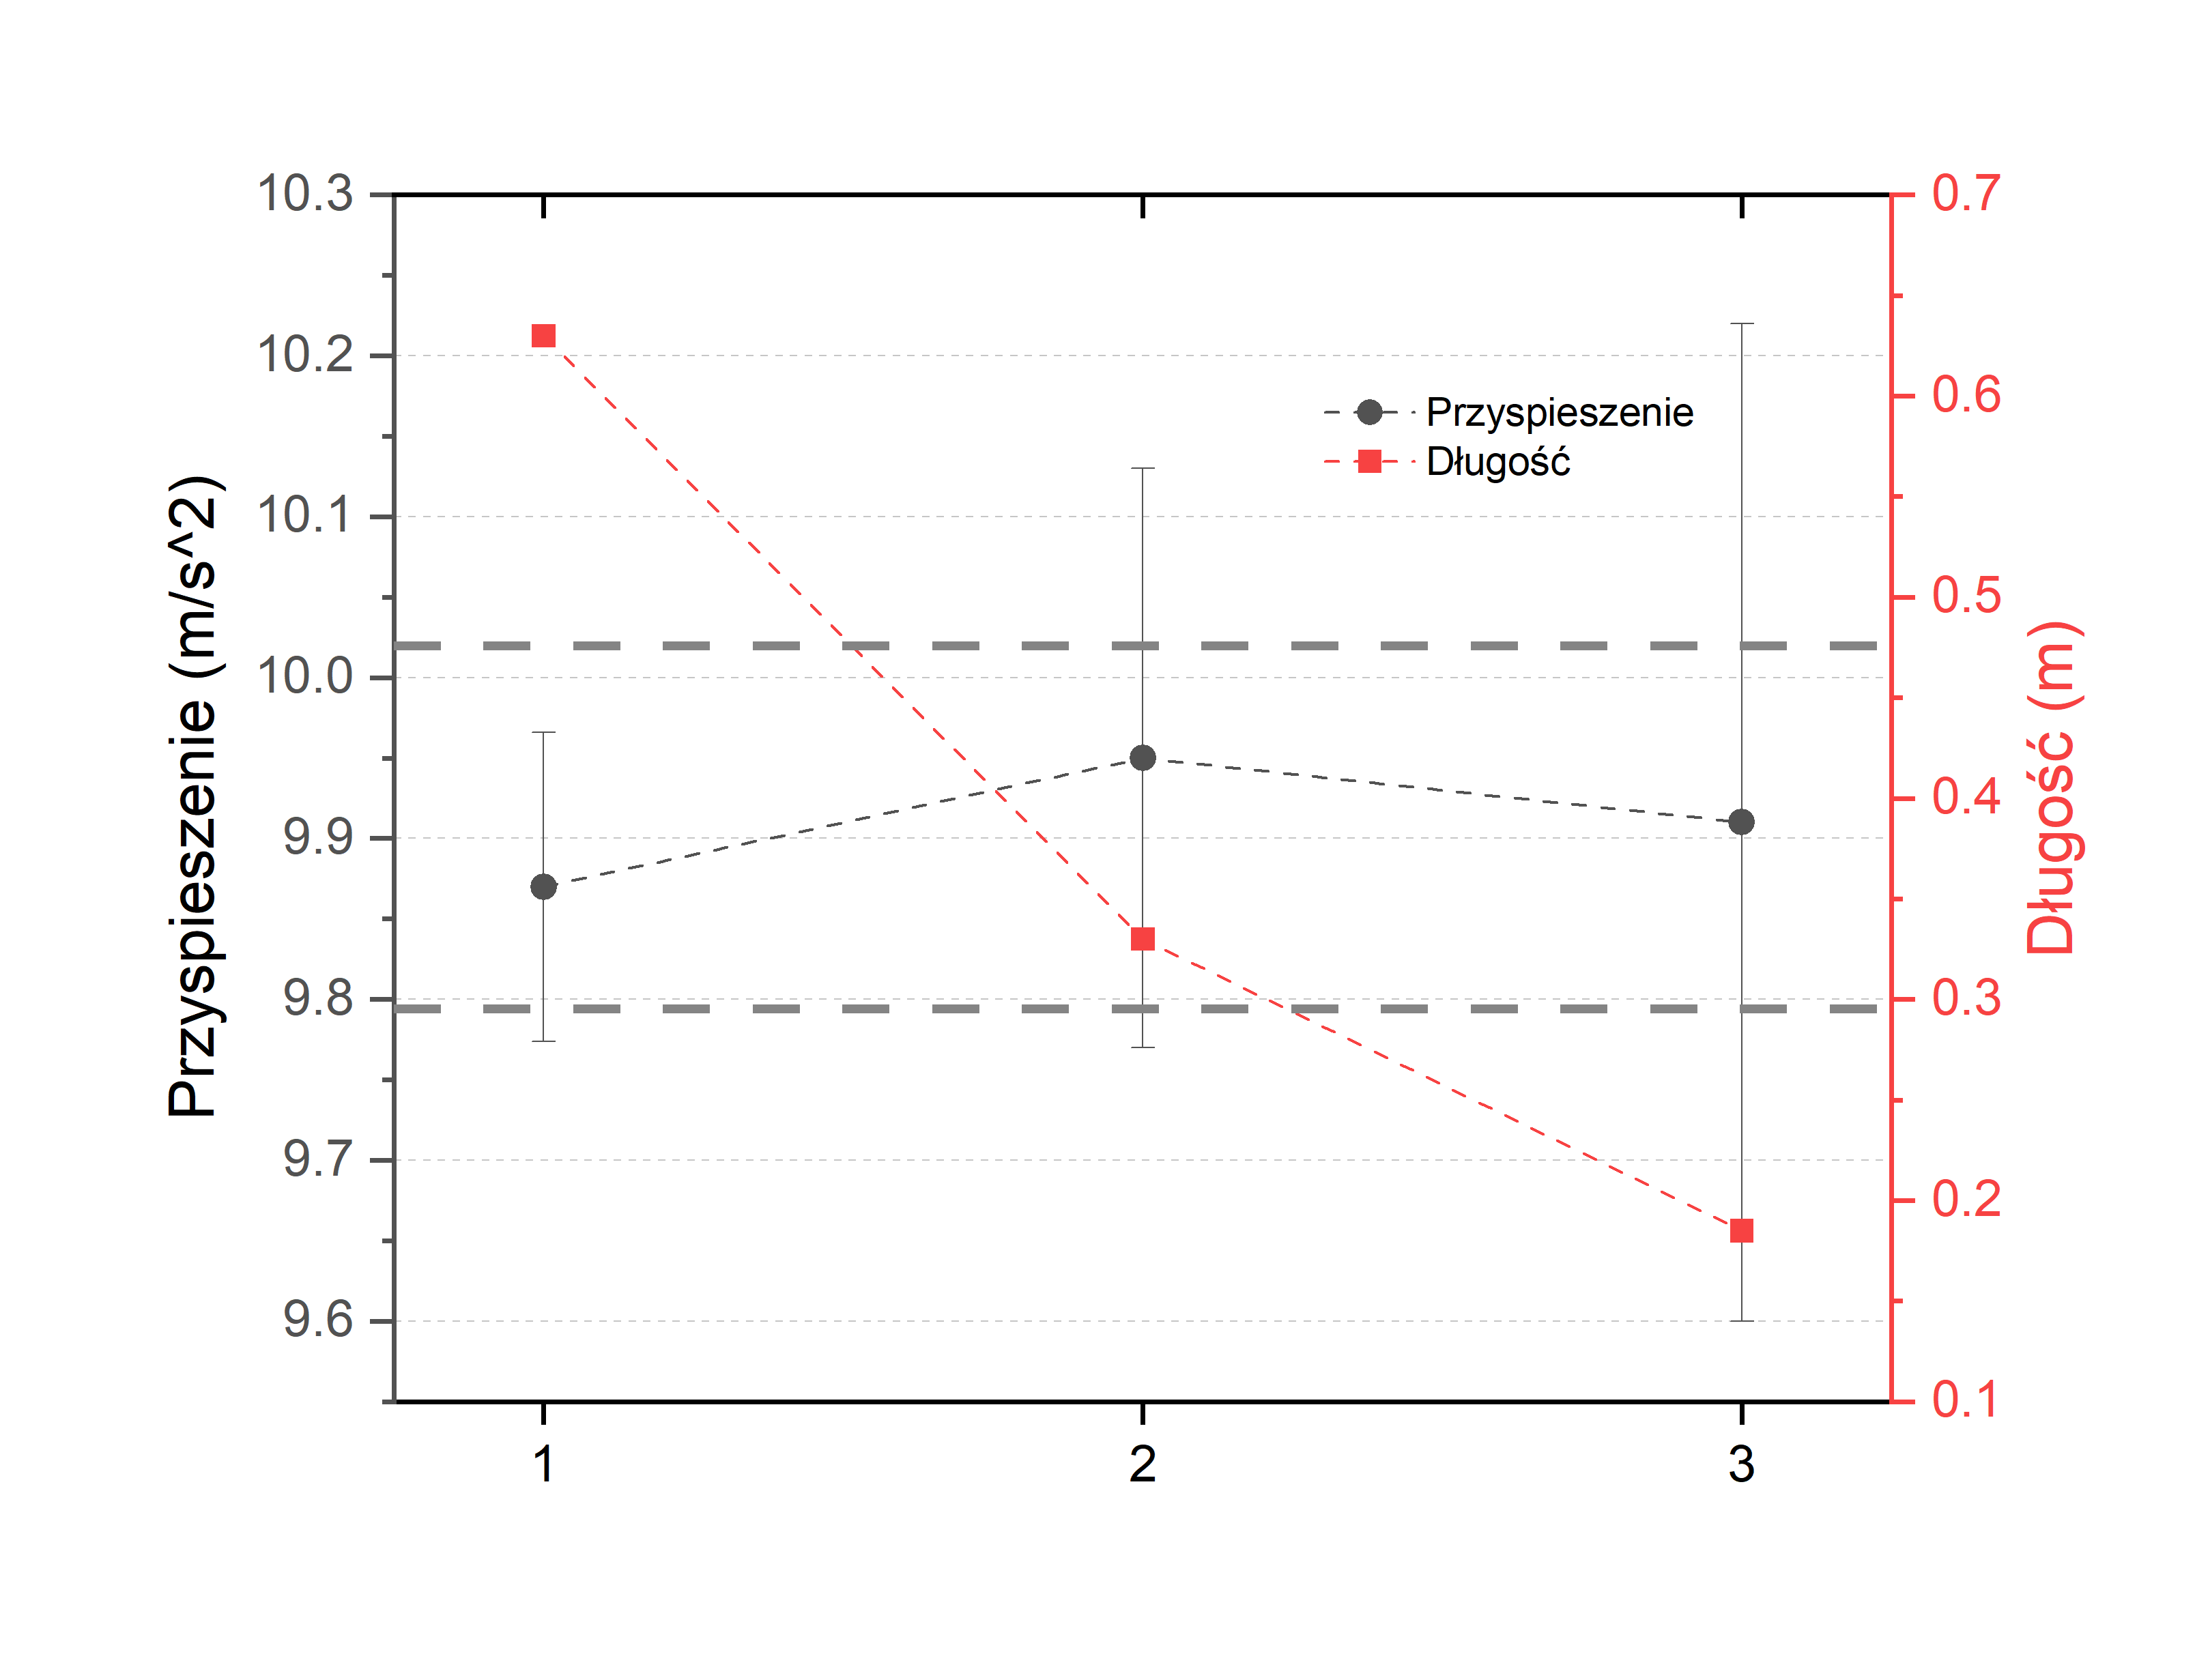
\includegraphics[width = 80mm]{imgs/Graph1.png}
    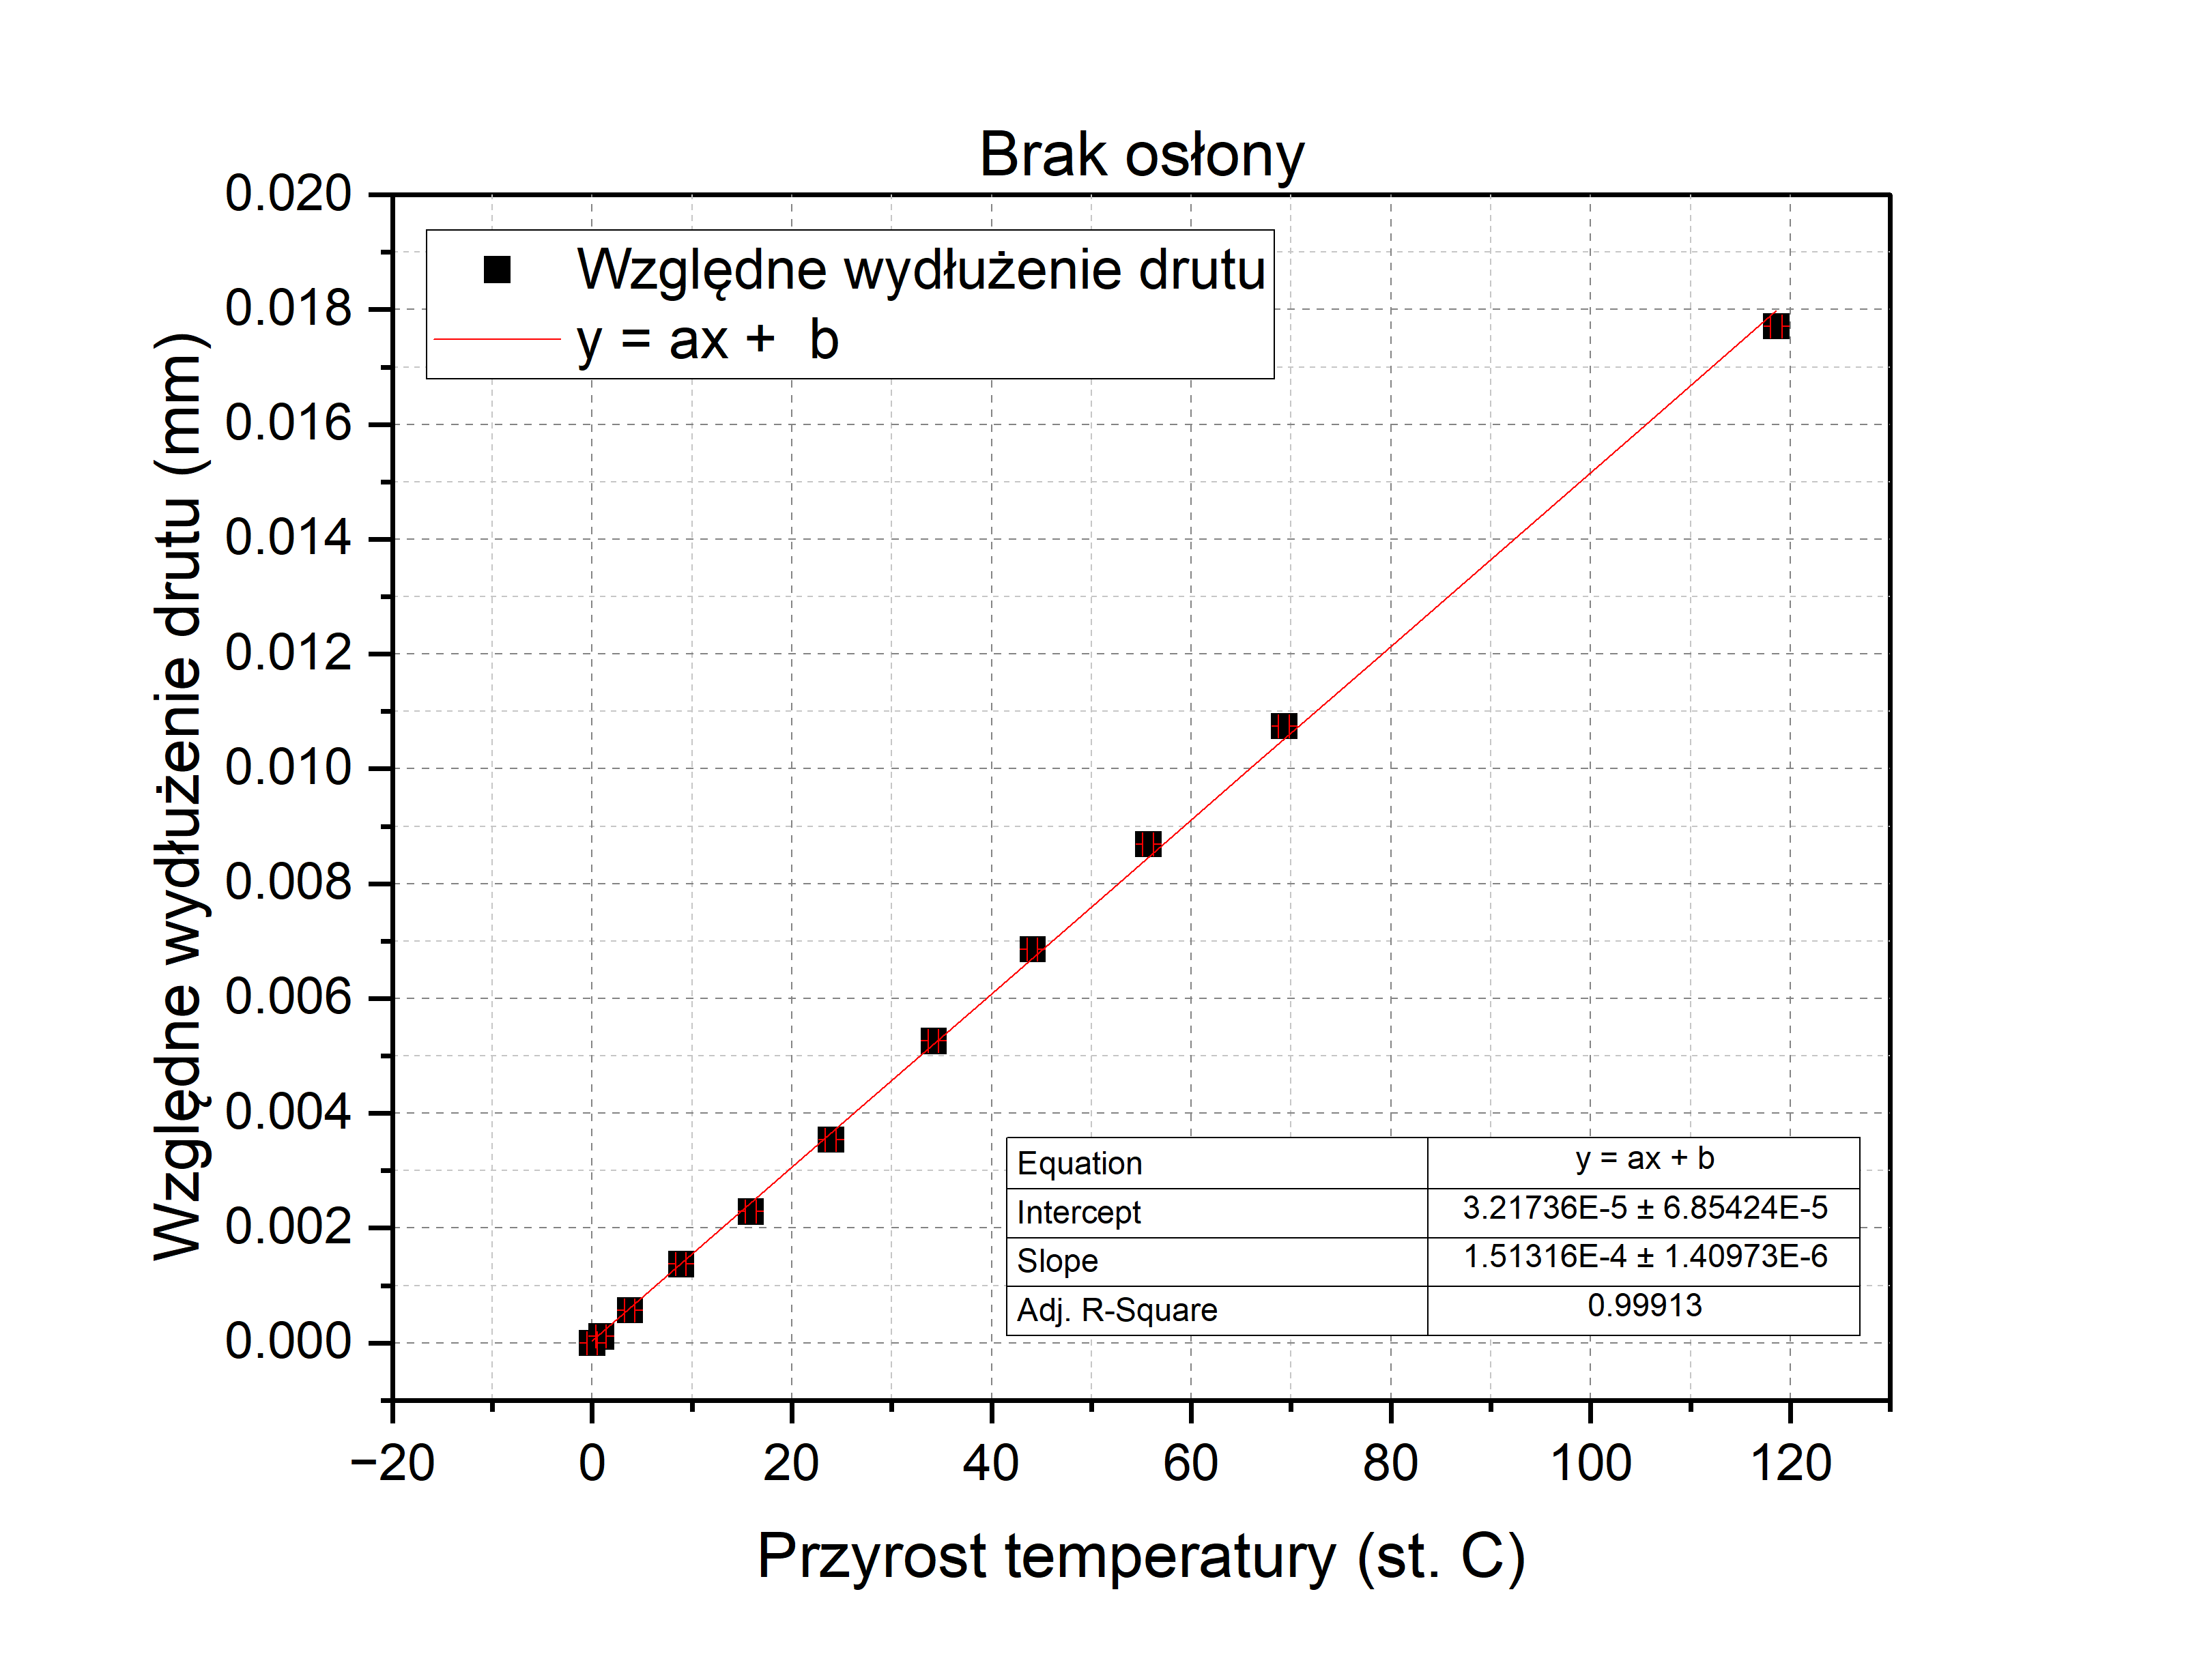
\includegraphics[width = 80mm]{imgs/Graph2.png}
    \label{fig:wykresy_dlugosci}
\end{figure}

Po wykonaniu regresji liniowej dla powyższych wykresów otrzymaliśmy współczynniki rozszerzalności termicznej. \\

\indent\indent Z osłoną   $\alpha = (1.52227 \pm 0.02865) \cdot 10^{-4} \frac{1}{^{\circ}C}$ \\
\indent\indent Bez osłony $\alpha = (1.51316 \pm 0.01410) \cdot 10^{-4} \frac{1}{^{\circ}C}$ \\

Do obliczenia mocy użyliśmy kolejnych pomiarów dokonywanych jednocześnie z poprzednimi.

\begin{center}
    \begin{tabular}{|c|c||c|c||c|c|}
        \hline
        \multicolumn{6}{|c|}{Pomiary z osłoną} \\
        \hline
        I    & u(I)   & U   & u(U)  & P      & u(P)    \\ \hline
        A    & A      & V   & V     & W      & W       \\ \hline
        0    & 0.01   & 0   & 0.01  & 0      & 0       \\ \hline
        0.19 & 0.0119 & 0.8 & 0.018 & 0.152  & 0.01012 \\ \hline
        0.39 & 0.0139 & 1.5 & 0.025 & 0.585  & 0.02302 \\ \hline
        0.6  & 0.016  & 2.3 & 0.033 & 1.38   & 0.04179 \\ \hline
        0.82 & 0.0182 & 3.1 & 0.041 & 2.542  & 0.06568 \\ \hline
        1.01 & 0.0201 & 3.8 & 0.048 & 3.838  & 0.09047 \\ \hline
        1.23 & 0.0223 & 4.7 & 0.057 & 5.781  & 0.1261  \\ \hline
        1.41 & 0.0241 & 5.4 & 0.064 & 7.614  & 0.15837 \\ \hline
        1.63 & 0.0263 & 6.3 & 0.073 & 10.269 & 0.20399 \\ \hline
        1.82 & 0.0282 & 7   & 0.08  & 12.74  & 0.24529 \\ \hline
        2.02 & 0.0302 & 7.8 & 0.088 & 15.756 & 0.29511 \\ \hline
    \end{tabular}
\end{center}

\begin{center}
    \begin{tabular}{|c|c||c|c||c|c|}
        \hline
        \multicolumn{6}{|c|}{Pomiary bez osłony} \\
        \hline
        I    & u(I)   & U   & u(U)  & P      & u(P)    \\ \hline
        A    & A      & V   & V     & W      & W       \\ \hline
        0    & 0.01   & 0   & 0.01  & 0      & 0       \\ \hline
        0.2  & 0.012  & 0.8 & 0.018 & 0.16   & 0.01025 \\ \hline
        0.4  & 0.014  & 1.5 & 0.025 & 0.6    & 0.02326 \\ \hline
        0.62 & 0.0162 & 2.4 & 0.034 & 1.488  & 0.04423 \\ \hline
        0.8  & 0.018  & 3.1 & 0.041 & 2.48   & 0.06473 \\ \hline
        1.01 & 0.0201 & 3.9 & 0.049 & 3.939  & 0.09271 \\ \hline
        1.21 & 0.0221 & 4.6 & 0.056 & 5.566  & 0.12217 \\ \hline
        1.41 & 0.0241 & 5.4 & 0.064 & 7.614  & 0.15837 \\ \hline
        1.62 & 0.0262 & 6.2 & 0.072 & 10.044 & 0.19998 \\ \hline
        1.82 & 0.0282 & 7   & 0.08  & 12.74  & 0.24529 \\ \hline
        2.4  & 0.034  & 9.3 & 0.103 & 22.32  & 0.40136 \\ \hline
    \end{tabular}
\end{center}

\newpage
\begin{figure}[!ht]
    \centering
    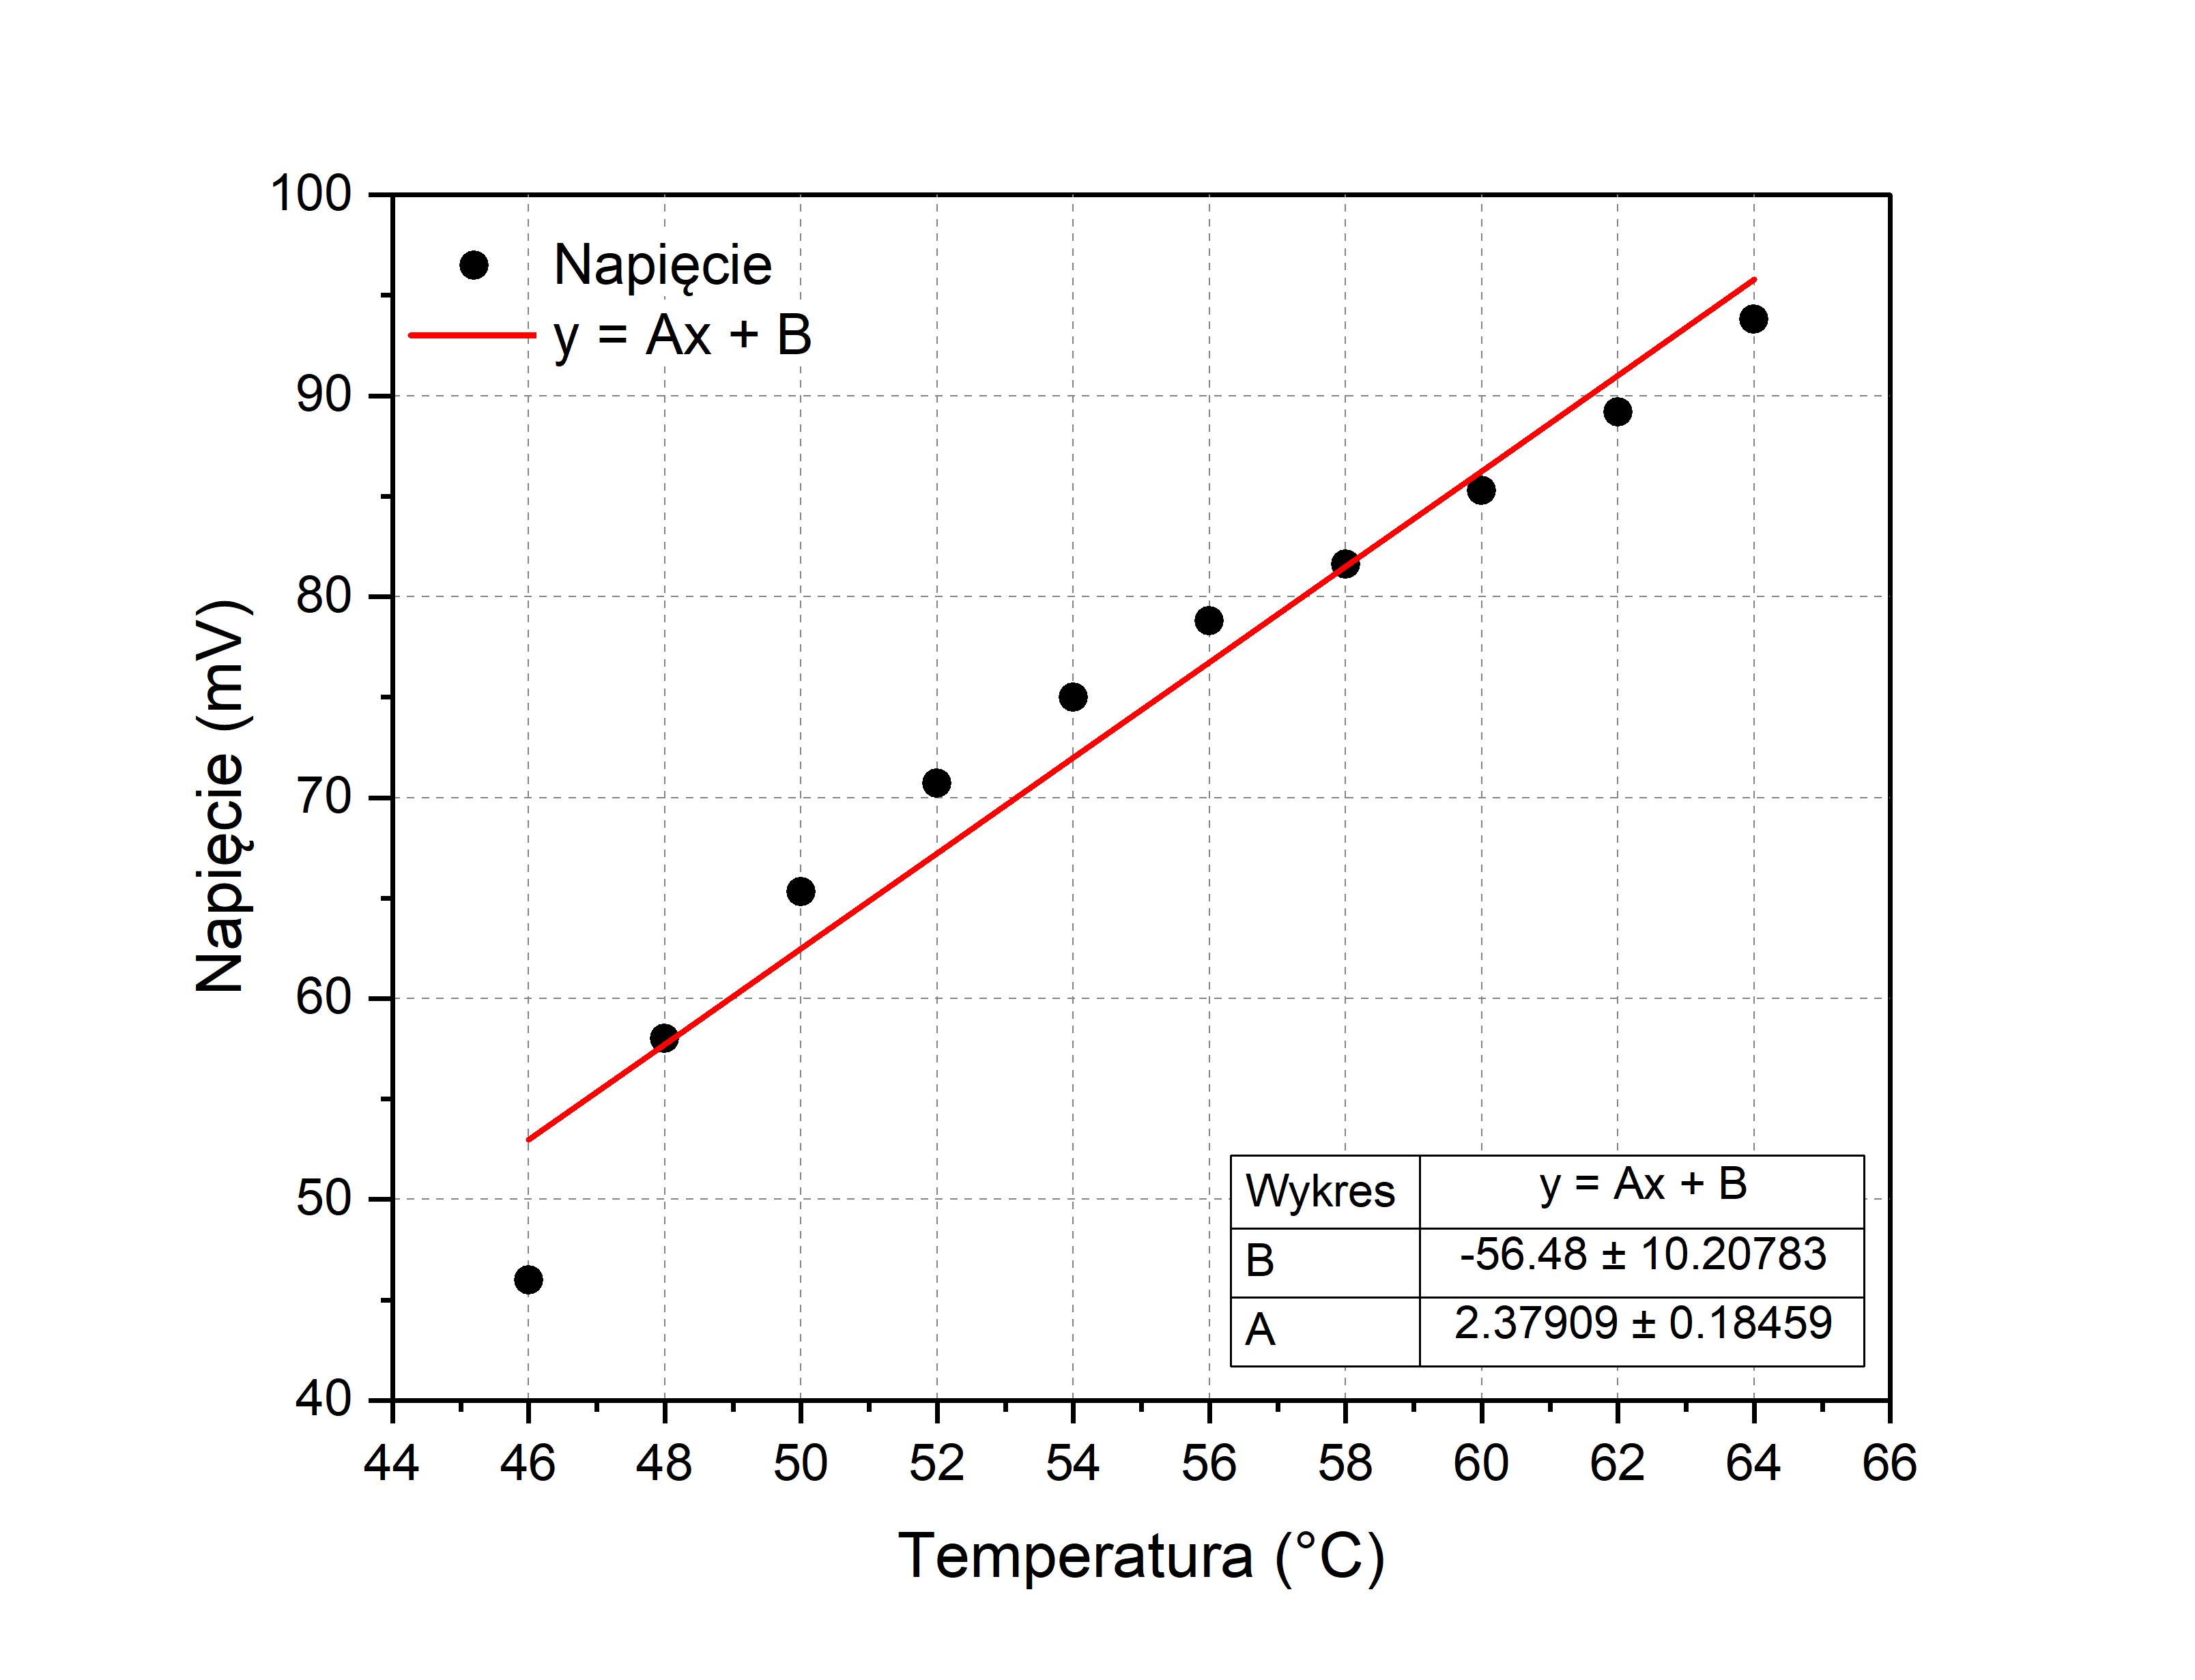
\includegraphics[width = 80mm]{imgs/Graph3.png}
    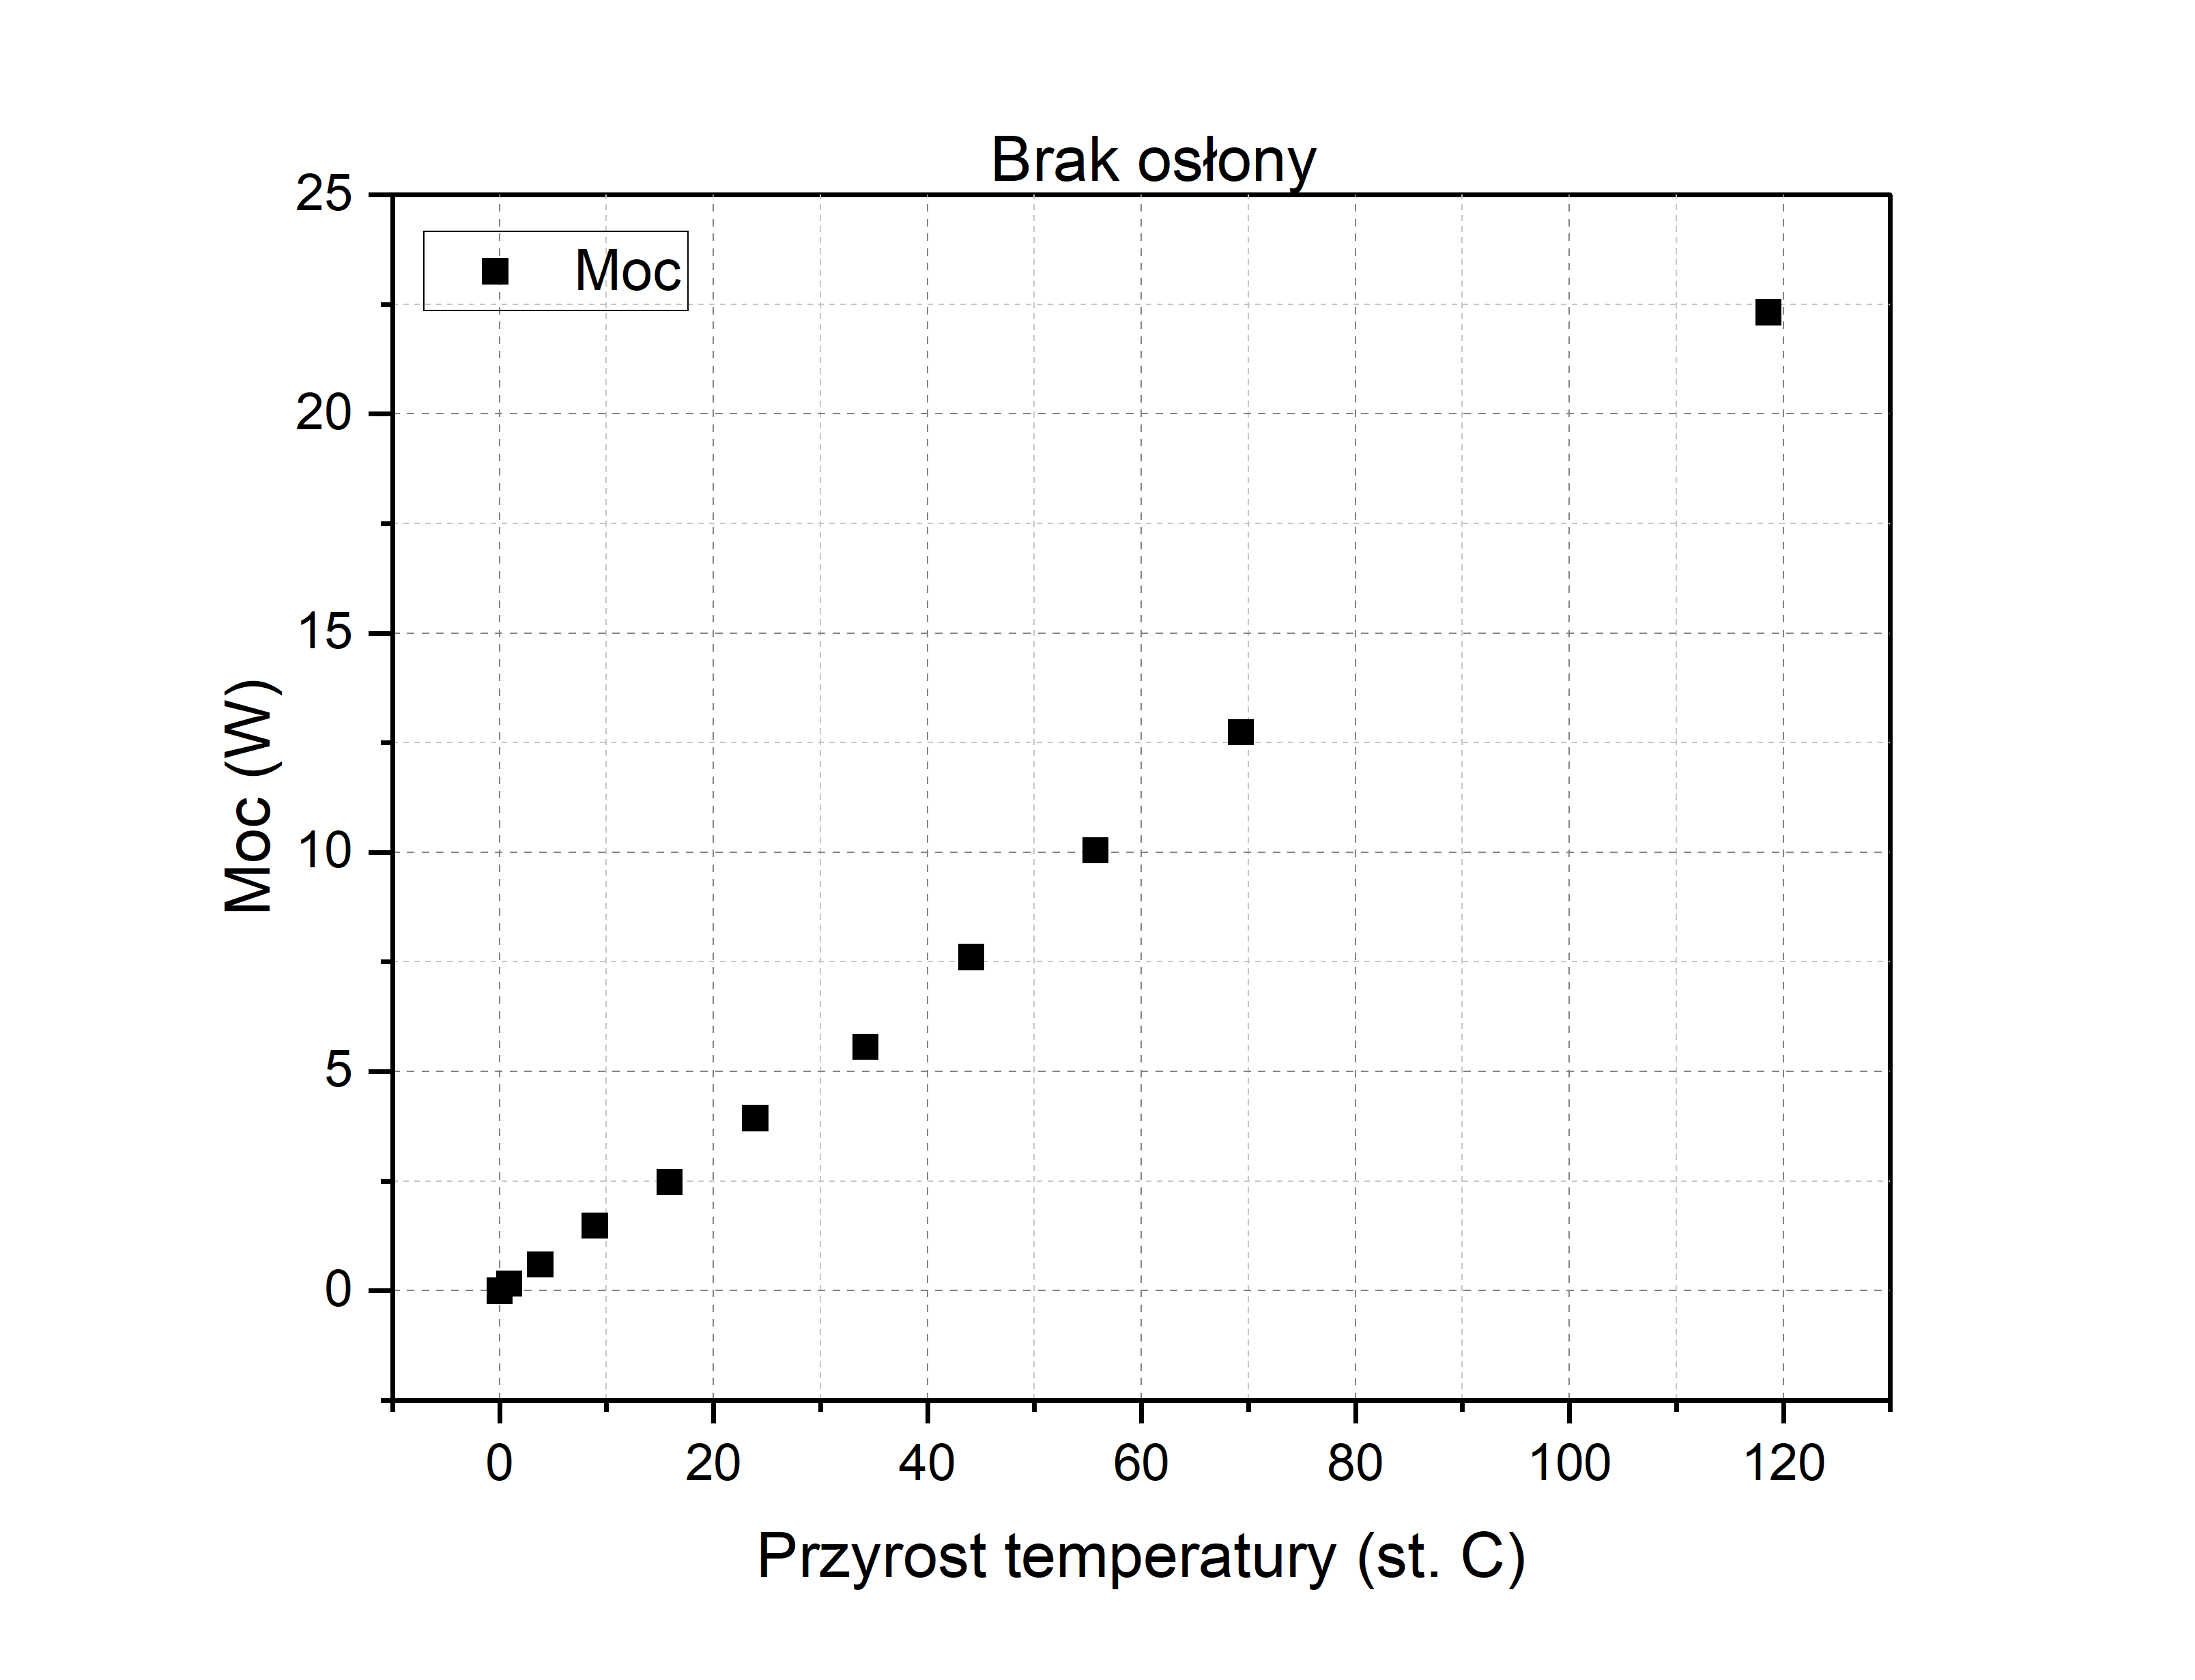
\includegraphics[width = 80mm]{imgs/Graph4.png}
    \label{fig:wykresy_mocy}
\end{figure}



\newpage
{\section{Wnioski}}

Ćwiczenie polegało na wyznaczeniu przyspieszenia ziemskiego stosując zależności między przyspieszeniem,
a obiektami fizycznymi. Ćwiczenie zostało wykonane poprawnie.\\

Średnia wartość przyspieszenia jaka została zmierzona za pomocą wahadła matematycznego w budynku A-1 w sali 54 wyniosła $g = 9.91 \frac{m}{s^2}$.

\begin{figure}[h]
    \centering
    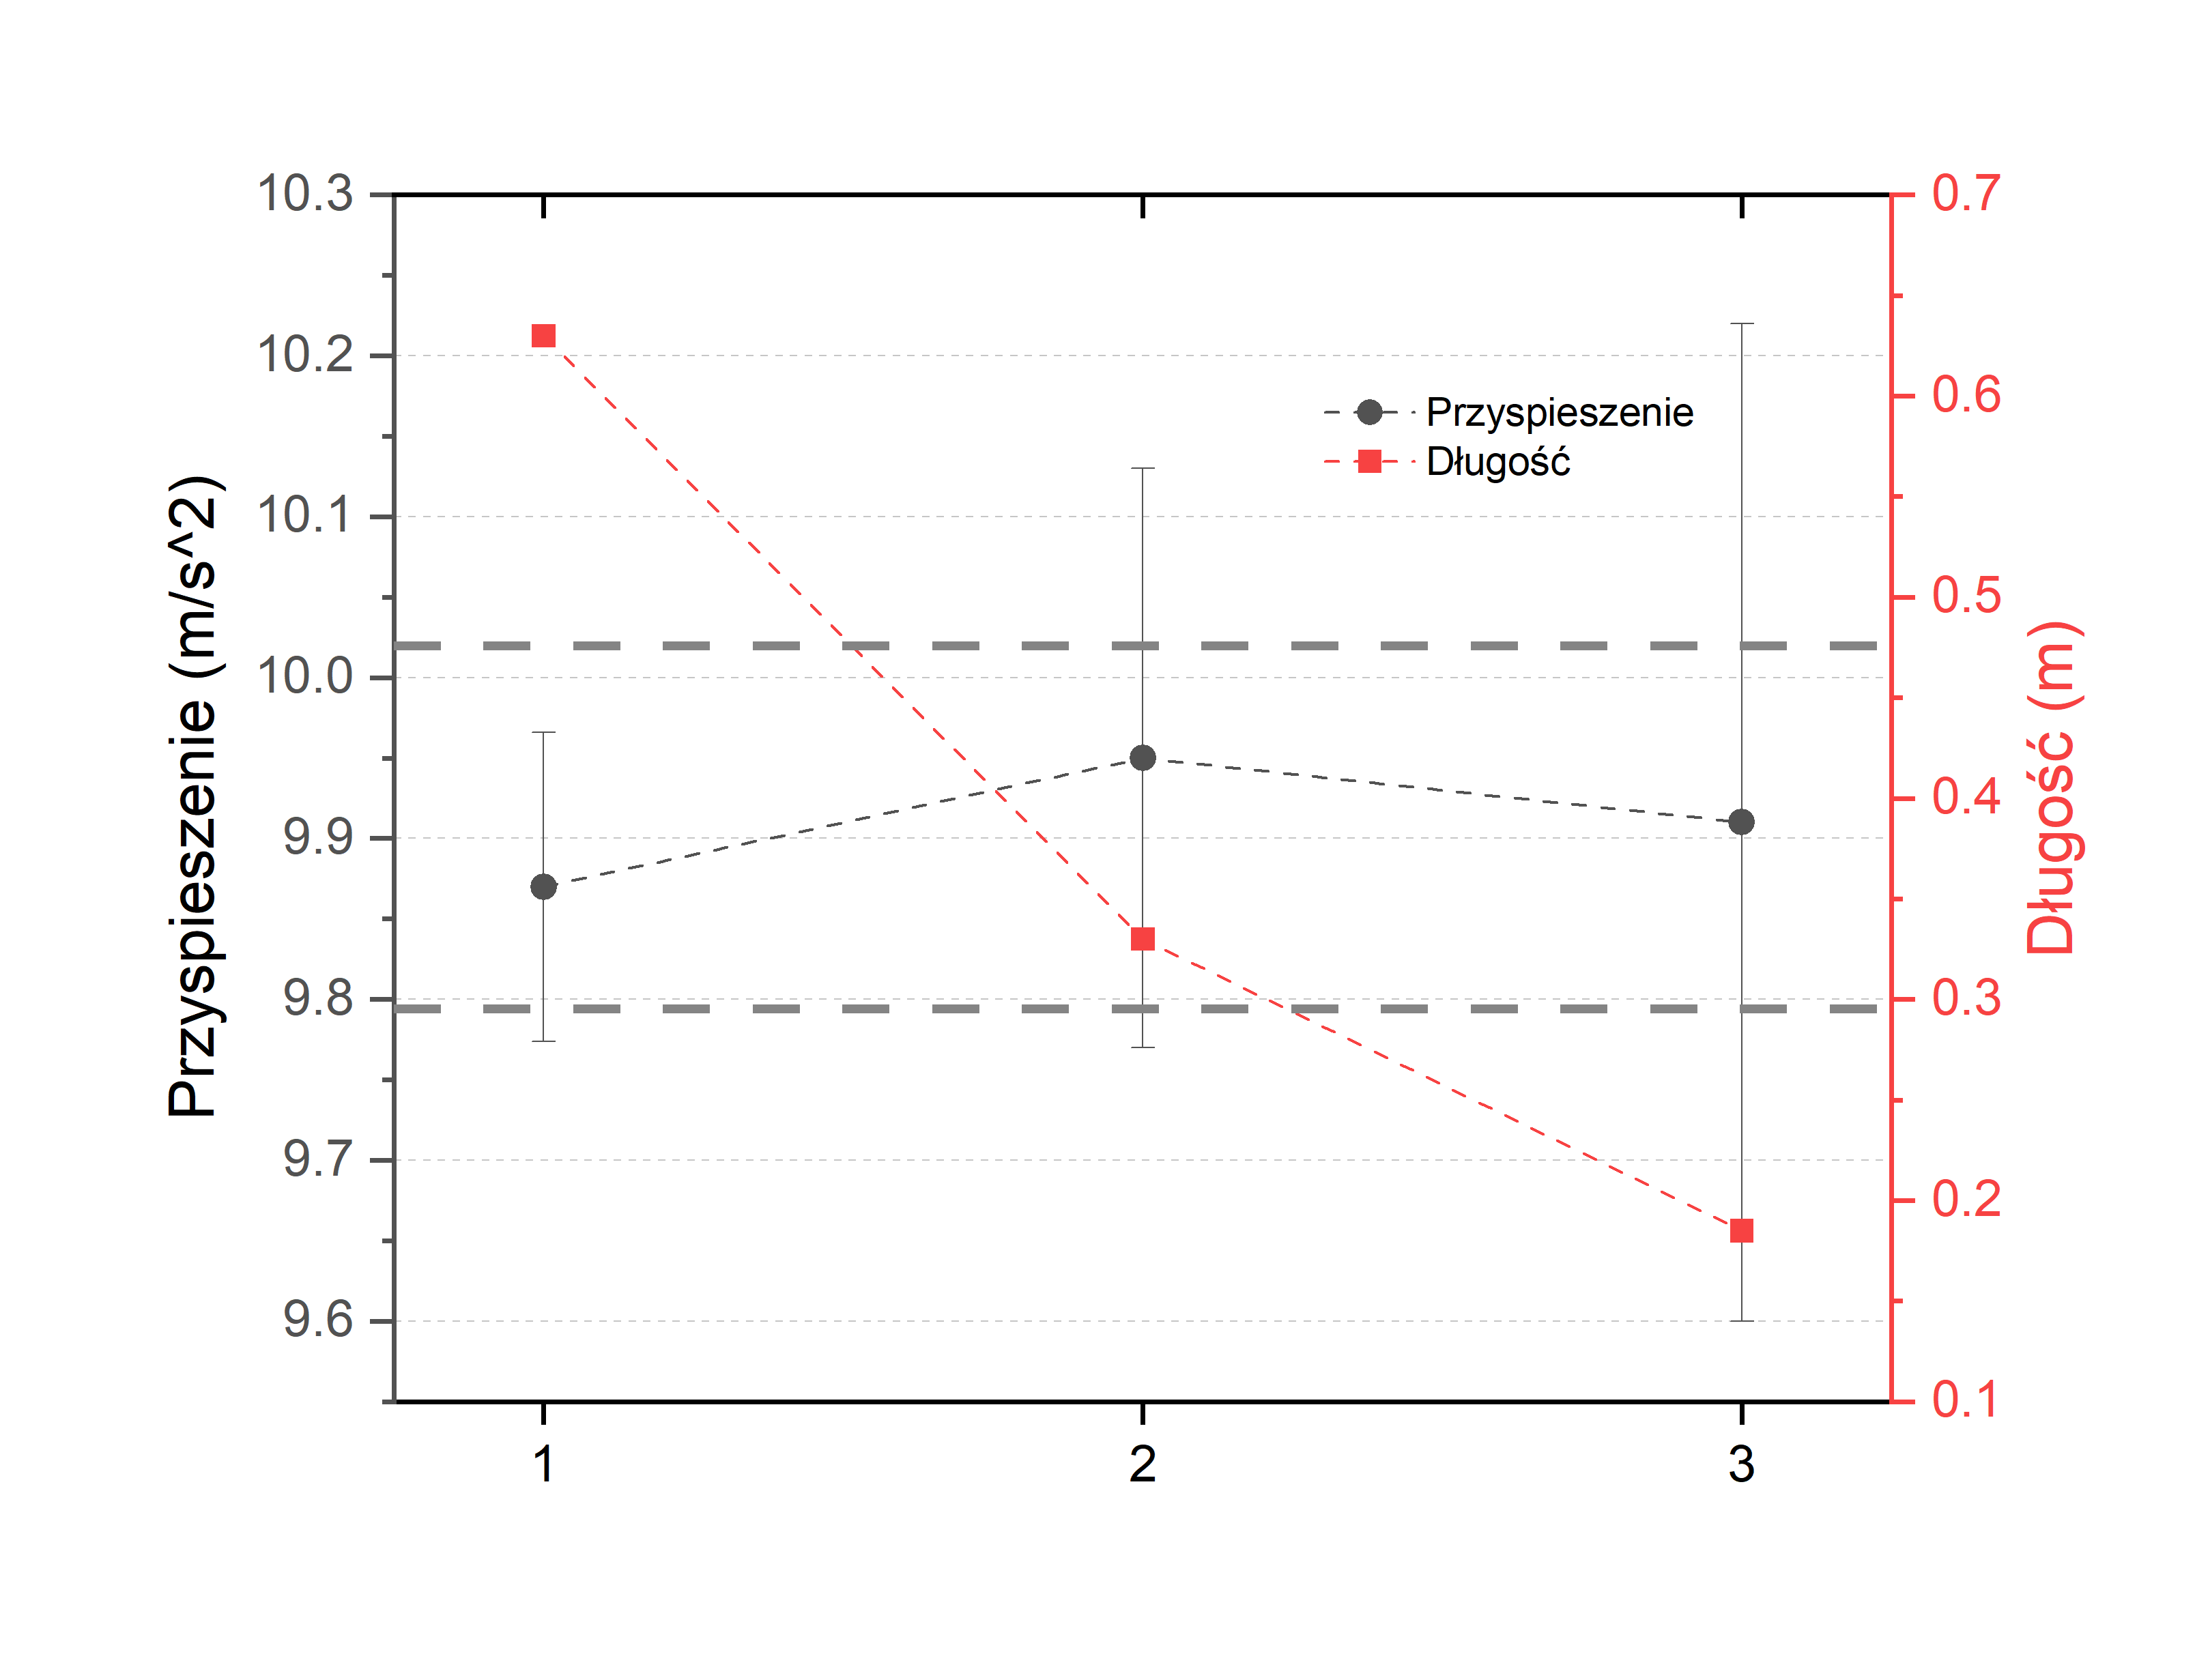
\includegraphics[width=100mm]{imgs/Graph1.png}
    \label{fig:wyniki_wm}
\end{figure}

Po zestawieniu obok siebie danych na wykresie można zauważyć pewną zależność między długością wahadła, a końcowym wynikiem ćwiczenia. Wszystkie 3 wyniki przyspieszenia ziemskiego dla poszczególnych długości wahadła mieszczą się w otoczeniu (niepewności) średniej ich wartości. Natomiast wraz ze skracaniem długości wahadła diametralnie wzrósła niepewność tego wyniku. Może to skutkować zbyt krótkim czasem oscylacji wahadła.

Wnioskujemy więc, że dla bardziej dokładnego wyniku przyspieszenia powinno się dokonywać doświadczenia stosując duże długości wahadła. Z zebranych danych wynika, że dla $l \leq 63cm$ otrzymamy dłuższe czasy oscylacji i większe uśrednienie okresu, co w efekcie końcowym da dokładniejszei wyniki przyspieszenia. \\

Średnia wartość przyspieszenia jaka została zmierzona za pomocą wahadła fizycznego w budynku A-1 w sali 54 wyniosła $g =10.26 \frac{m}{s^2}$.\\

Porównując te wyniki możemy wyciągnąć wniosek, że wahadło matematyczne  jest dokładniejszym narzędziem do wyznaczania wartości przyciągania grawitacyjnego.


\end{document}
